\rhschapter{Object Orienteret Design}

\section{Gameplay}
Unreal Breakout er et spil med et bat\footnote{Paddle på engelsk, bliver brugt i vores paddle klasse.}, en bold\footnote{Ball på engelsk, bliver brugt i vores ball klasse.}, en masse brikker\footnote{Bricks på engelsk, bliver brugt i vores bricks klasse.}, tre lukkede sidder, og en åben side i bunden. Formålet med spillet er at få bolden til at ramme alle brikkerne og sørge for at bolden ikke ryger ud af banen i bunden hvor spillerens bat og den åbne side er. Når man rammer en brik, går den i stykker eller skifter farve, når en brik rammes vil der blive tilføjet point til spillerens score. Når spillet starter har man 3 liv(bolde) og bolden er låst fast på spillerens bat nederst i midten af skærmen. Når man trykker på en dertil bestemt knap skyder man bolden afsted, og med nogle andre knapper bevæger man battet fra side til side for at undgå at bolden ryger ud af spilområdet. Hvis bolden ryger ud af spilområdet, mister man et liv(bold) og en ny bold bliver låst fast til battet og er klar til at blive skudt afsted. Når spilleren har mistet alle liv og den sidste bold ryger ud af spilområdet, slutter spillet. Får man til gengæld fjernet alle brikker, vindes banen og den samme bane kommer igen uden at ændre på antal liv spilleren har tilbage eller nulstille scoren, og bolden bliver igen fastlåst til battet.

\section{Grafik} 

Spillets grafik er fundet på \textit{opengameart.org}, som er en hjemmeside hvor folk lægger grafik op til fri afbenyttelse. Dette betyder at det er uden licens men man kan dog donere penge til de brugere der har lagt grafikken tilgængelig på siden. Nogle af grafikerne på siden vil dog gerne have deres navn nævnt hvis deres grafik bruges. \newline
Breakout er et gammelt spil udviklet af Atari, derfor er der fundet grafik som er tro mod det klassiske spils grafik. Grafikken ligger på nogle spritesheets som er kollager af billeder som bliver brugt til at skabe de forskellige elementer i spillet. Når spritesheetet er delt op vil de forskellige brikker blive bygget op til en bane. Eftersom spilleren rammer brikkerne med bolden vil de skifte farve, farverne indikere hvor mange gange en brik skal rammes for at blive ødelagt. De grafiske elementer er ikke noget der vil blive sat stor fokus på i spillet, da det er spillets gameplay der skal være grundpillen i det. 

\section{Blueprints}
Blueprints er en speciel type asset som giver en node baseret interface til at lave nye klasser og udvide klasser, så man kan scripte objekter i levels og widgets. Blueprints er et værktøj der giver designers og gameplay-programmører mulighed for hurtigt at kunne udvikle deres idéer uden at skulle skrive kode.

Det er stadig muligt selv at oprette klasser med C++ kode uden at bruge blueprints. Blueprints kan bruges til at udvide klasser som er skrevet i C++, gemme og modificere properties og håndtere objektinstanser i klasser.

Ligesom i C++ og C\# har blueprints member variables/fields, member functions, og en constructor.

\begin{list}{}{}
\item[Der er 3 typer Blueprints:]
\item[Blueprint Class]
\item[Data-Only Blueprint]
\item[Level Blueprint]
\end{list}

Blueprint Class er det blueprint man bruger når man vil have et objekt til at gøre noget inde i et \textit{level}. Man laver noget funktionalitet i dette blueprint og tilføjer det til et objekt i et \textit{level}. Data-Only Blueprints indeholder kun nodes, variabler og komponenter som det har nedarvet og der kan ikke tilføjes nyt. Det den bruges til er at ændre på objekter i et \textit{level} og lave variationer som alle har samme interface, men forskellig adfærd. Level Blueprint er et blueprint som altid findes når man opretter et nyt \textit{level}. Det er et overordnet blueprint som eksisterer sammen med de Blueprints som sidder på objekter i banen. Man kan bruge Level Blueprint til at oprette events som andre objekters blueprints kan agere på. Man kan også oprette instanser af andre assets gennem Level Blueprint, som f.eks. et UI der skal tegnes i Camera Actor'en i banen. Se \cite{blueprint} for mere information.

I figur \ref{dia:codeblueprint1} kan ses et simpelt eksempel på hvordan noder kan sættes sammen i et blueprint. I eksemplet sættes to \textit{private int} variabler til to forskellige tal og derefter bliver de lagt sammen og sat i en tredje \textit{private int} variabel. Når man opretter variabler i et blueprint er de ligesom fields i C\# hvor de kan defineres som private eller public. Forskellen er at blueprints altid initialiserer variabler med en standard værdi, hvor man i C\# kode godt kan lade variabler være uinitialiserede.

Hvis man oversætter noderne fra blueprint eksemplet i figur \ref{dia:codeblueprint1} til for C\# kode, vil det være noget lignende koden i figur \ref{dia:codeblueprint2}. Unreal Engine 4 er lavet med C++ kode og alle noderne i blueprints omsættes også til C++ kode. Det er derfor at man skal \textit{compile} hver gang man laver ændringer i noderne. Vi er ikke klar over hvordan det præcist ser ud når Unreal Engine 4 compiler et blueprint om til en klasse i C++, men vi er ret sikker på at der bliver oprettet et par hjælpe metoder og variabler i dem for at \textit{game engine}'en kan holde styr på det hele. Der er for eksempel et \textit{BeginPlay} event man kan gøre brug af i editoren og et \textit{EventTick} event.

\begin{figure}
	\begin{center}
		\caption{Simpelt eksempel på noder i blueprints.}
		\label{dia:codeblueprint1}
		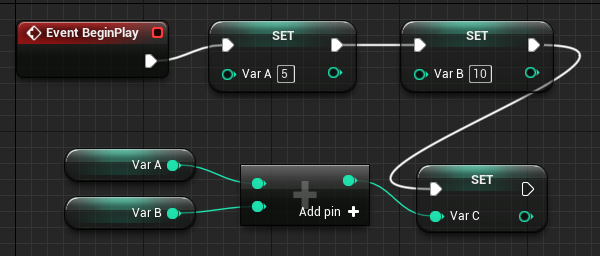
\includegraphics[width=0.80\linewidth]{pictures/blueprints/blueprint-example}
		\end{center}
\end{figure}

\begin{figure}
\caption{C\# kode eksempel på noder i blueprints.}
\label{dia:codeblueprint2}
\begin{lstlisting}
using System;

public class ExampleClass
{
    private int VarA = 0;
    private int VarB = 0;
    private int VarC = 0;

    public ExampleClass()
    {
    }
    
    public void BeginPlay()
    {
        VarA = 5;
        VarB = 10;
        VarC = VarA + VarB;
    }
}
\end{lstlisting}
\end{figure}